% Options for packages loaded elsewhere
\PassOptionsToPackage{unicode}{hyperref}
\PassOptionsToPackage{hyphens}{url}
\PassOptionsToPackage{dvipsnames,svgnames,x11names,table}{xcolor}
\documentclass[
  spanish,
  a4paper,
  11pt
]{article}
\usepackage{xcolor}
\usepackage[margin=22mm, top=26mm, bottom=26mm]{geometry}
\usepackage{amsmath,amssymb}
\setcounter{secnumdepth}{2} % numeración clara de secciones

\usepackage{iftex}
\ifPDFTeX
  \usepackage[T1]{fontenc}
  \usepackage[utf8]{inputenc}
  \usepackage{textcomp}
\else
  \usepackage{unicode-math}
  \defaultfontfeatures{Scale=MatchLowercase}
  \defaultfontfeatures[\rmfamily]{Ligatures=TeX,Scale=1}
\fi
\usepackage{lmodern}

% Paquetes de diseño profesional
\usepackage{fancyhdr}
\usepackage{titlesec}
\usepackage{tcolorbox}
\tcbuselibrary{skins,breakable}
\usepackage{colortbl}
\usepackage{booktabs}
\usepackage{tabularx}
\usepackage{enumitem}
\usepackage{caption}
\AtBeginDocument{\renewcommand{\figurename}{Figura}\renewcommand{\tablename}{Tabla}}

% Paleta de Colores Institucional & Técnica
\definecolor{UPSEBlue}{RGB}{11, 59, 96}
\definecolor{DarkNavy}{RGB}{15, 23, 42}
\definecolor{AccentCyan}{RGB}{2, 132, 199}
\definecolor{PassGreen}{RGB}{22, 163, 74}
\definecolor{FailRed}{RGB}{220, 38, 38}
\definecolor{LightGrayBg}{RGB}{248, 250, 252}
\definecolor{BorderGray}{RGB}{226, 232, 240}
\definecolor{CodeBg}{RGB}{241, 245, 249}

% Estilo de Encabezados y Pies de Página
\newcommand{\codebreak}{\allowbreak}
\providecommand{\tightlist}{\setlength{\itemsep}{0pt}\setlength{\parskip}{0pt}}
\setlength{\headheight}{22pt}
\renewcommand{\contentsname}{Contenido}
\newcommand{\evid}[1]{\href{https://github.com/yan2005dris-afk/SDCC---microservices-with-gateway-and-loadbalancer/blob/70ee0a32947f29515b9d0ab2961b1314c0b0938c/docs/evidencias/#1}{\texttt{#1}}}
\pagestyle{fancy}
\fancyhf{}
\renewcommand{\headrulewidth}{0.6pt}
\renewcommand{\footrulewidth}{0.4pt}
\renewcommand{\headrule}{\hbox to\headwidth{\color{UPSEBlue}\leaders\hrule height \headrulewidth\hfill}}
\fancyhead[L]{\small\color{UPSEBlue}\textbf{UPSE · Aplicaciones Distribuidas}}
\fancyhead[R]{\small\color{gray}Informe Experimental P01--P08}
\fancyfoot[L]{\footnotesize\color{gray}SDCC --- Microservicios con Gateway y LoadBalancer}
\fancyfoot[R]{\small\color{UPSEBlue}\textbf{Página \thepage}}

% Estilo de Secciones y Títulos
\titleformat{\section}
  {\color{UPSEBlue}\Large\bfseries}
  {\thesection.}{0.8em}{}[\titlerule]
\titleformat{\subsection}
  {\color{DarkNavy}\large\bfseries}
  {\thesubsection}{0.6em}{}
\titleformat{\subsubsection}
  {\color{AccentCyan}\normalsize\bfseries}
  {\thesubsubsection}{0.5em}{}

% Cajas de Destaque Callout
\newtcolorbox{infobox}[1][]{
  enhanced,
  colback=LightGrayBg,
  colframe=UPSEBlue,
  arc=3mm,
  left=14pt,
  right=14pt,
  top=10pt,
  bottom=10pt,
  boxrule=1.2pt,
  title=\textbf{#1},
  coltitle=white,
  fonttitle=\bfseries\small,
  attach boxed title to top left={yshift=-2mm, xshift=10pt},
  boxed title style={colback=UPSEBlue, arc=1.5mm}
}

\newtcolorbox{alertbox}[1][]{
  enhanced,
  colback=red!5!white,
  colframe=FailRed,
  arc=3mm,
  left=14pt,
  right=14pt,
  top=10pt,
  bottom=10pt,
  boxrule=1.2pt,
  title=\textbf{#1},
  coltitle=white,
  fonttitle=\bfseries\small,
  attach boxed title to top left={yshift=-2mm, xshift=10pt},
  boxed title style={colback=FailRed, arc=1.5mm}
}

% Listados y espaciados
\setlist[itemize]{noitemsep, topsep=4pt}
\setlist[enumerate]{noitemsep, topsep=4pt}

% Enlaces
\usepackage{bookmark}
\IfFileExists{xurl.sty}{\usepackage{xurl}}{}
\urlstyle{same}
\hypersetup{
  pdflang={es},
  colorlinks=true,
  linkcolor={UPSEBlue},
  filecolor={UPSEBlue},
  citecolor={AccentCyan},
  urlcolor={AccentCyan},
  pdfcreator={LaTeX - SDCC Distribuidos}}

\begin{document}

% PORTADA MODERNA INSTITUCIONAL
\begin{titlepage}
\begin{center}
  \vspace*{-1cm}
  
\includegraphics[width=42mm]{UPSELogo.png}\\[1.2em]
  {\Large\bfseries\color{UPSEBlue} UNIVERSIDAD ESTATAL PENÍNSULA DE SANTA ELENA}\\[0.4em]
  {\large\color{gray} FACULTAD DE SISTEMAS Y TELECOMUNICACIONES}\\[0.3em]
  {\normalsize\color{gray} CARRERA DE TECNOLOGÍAS DE LA INFORMACIÓN}\\[0.5em]
  \noindent\rule{0.8\textwidth}{0.8pt}\\[1.5em]

  {\large\bfseries\color{AccentCyan} APLICACIONES DISTRIBUIDAS}\\[1.8em]

  {\huge\bfseries\color{DarkNavy} Microservicios con Descubrimiento Dinámico, Balanceo de Carga y Persistencia Replicada}\\[1em]
  {\Large\color{UPSEBlue}\bfseries Informe Experimental de Pruebas P01 a P08}\\[2.5em]

  \begin{tcolorbox}[
    enhanced,
    colback=LightGrayBg,
    colframe=BorderGray,
    arc=4mm,
    width=0.88\textwidth,
    boxrule=1pt,
    drop shadow=black!10!white
  ]
    \centering
    \vspace{0.4em}
    {\bfseries\color{DarkNavy}\large Equipo de Investigación y Desarrollo}\\[0.8em]
    \renewcommand{\arraystretch}{1.3}
    \begin{tabular}{ll}
      \textbf{Yandris Rivera Torres} & \small Arquitectura y Descubrimiento Eureka (P01) \\
      \textbf{Gino Bermúdez} & \small Balanceo de Carga y LoadBalancer (P02) \\
      \textbf{Allison Reyes} & \small Transacciones e Inventario (P04, P05, P07) \\
      \textbf{Andy Alejandro} & \small Tolerancia a Fallos y Failover (P03, P06, P08) \\
    \end{tabular}
    \vspace{0.4em}
  \end{tcolorbox}

  \vfill
  {\normalsize\color{gray} La Libertad, Santa Elena, Ecuador}\\[0.3em]
  {\bfseries\color{DarkNavy} Noviembre 2026}
\end{center}
\end{titlepage}

\newpage
\thispagestyle{fancy}
{
  \hypersetup{linkcolor=DarkNavy}
  \tableofcontents
}
\newpage

\section{Arquitectura evaluada}\label{arquitectura-evaluada}

El cliente accede a Spring Cloud Gateway por el puerto 8080. El Gateway
usa Eureka, publicado en el puerto 8761, y Spring Cloud LoadBalancer
para dirigir solicitudes a las dos instancias de Pedidos y al servicio
de Inventario. Pedidos reserva stock mediante una llamada HTTP a
Inventario por su nombre lógico. Cada servicio usa su propia base
lógica.

PostgreSQL tiene un primario y dos réplicas físicas por streaming WAL
asíncrono. Pedidos envía las escrituras y lecturas críticas al primario
y distribuye las lecturas ordinarias entre réplicas aptas. Inventario
opera contra el primario.

\begin{figure}[htbp]
  \centering
  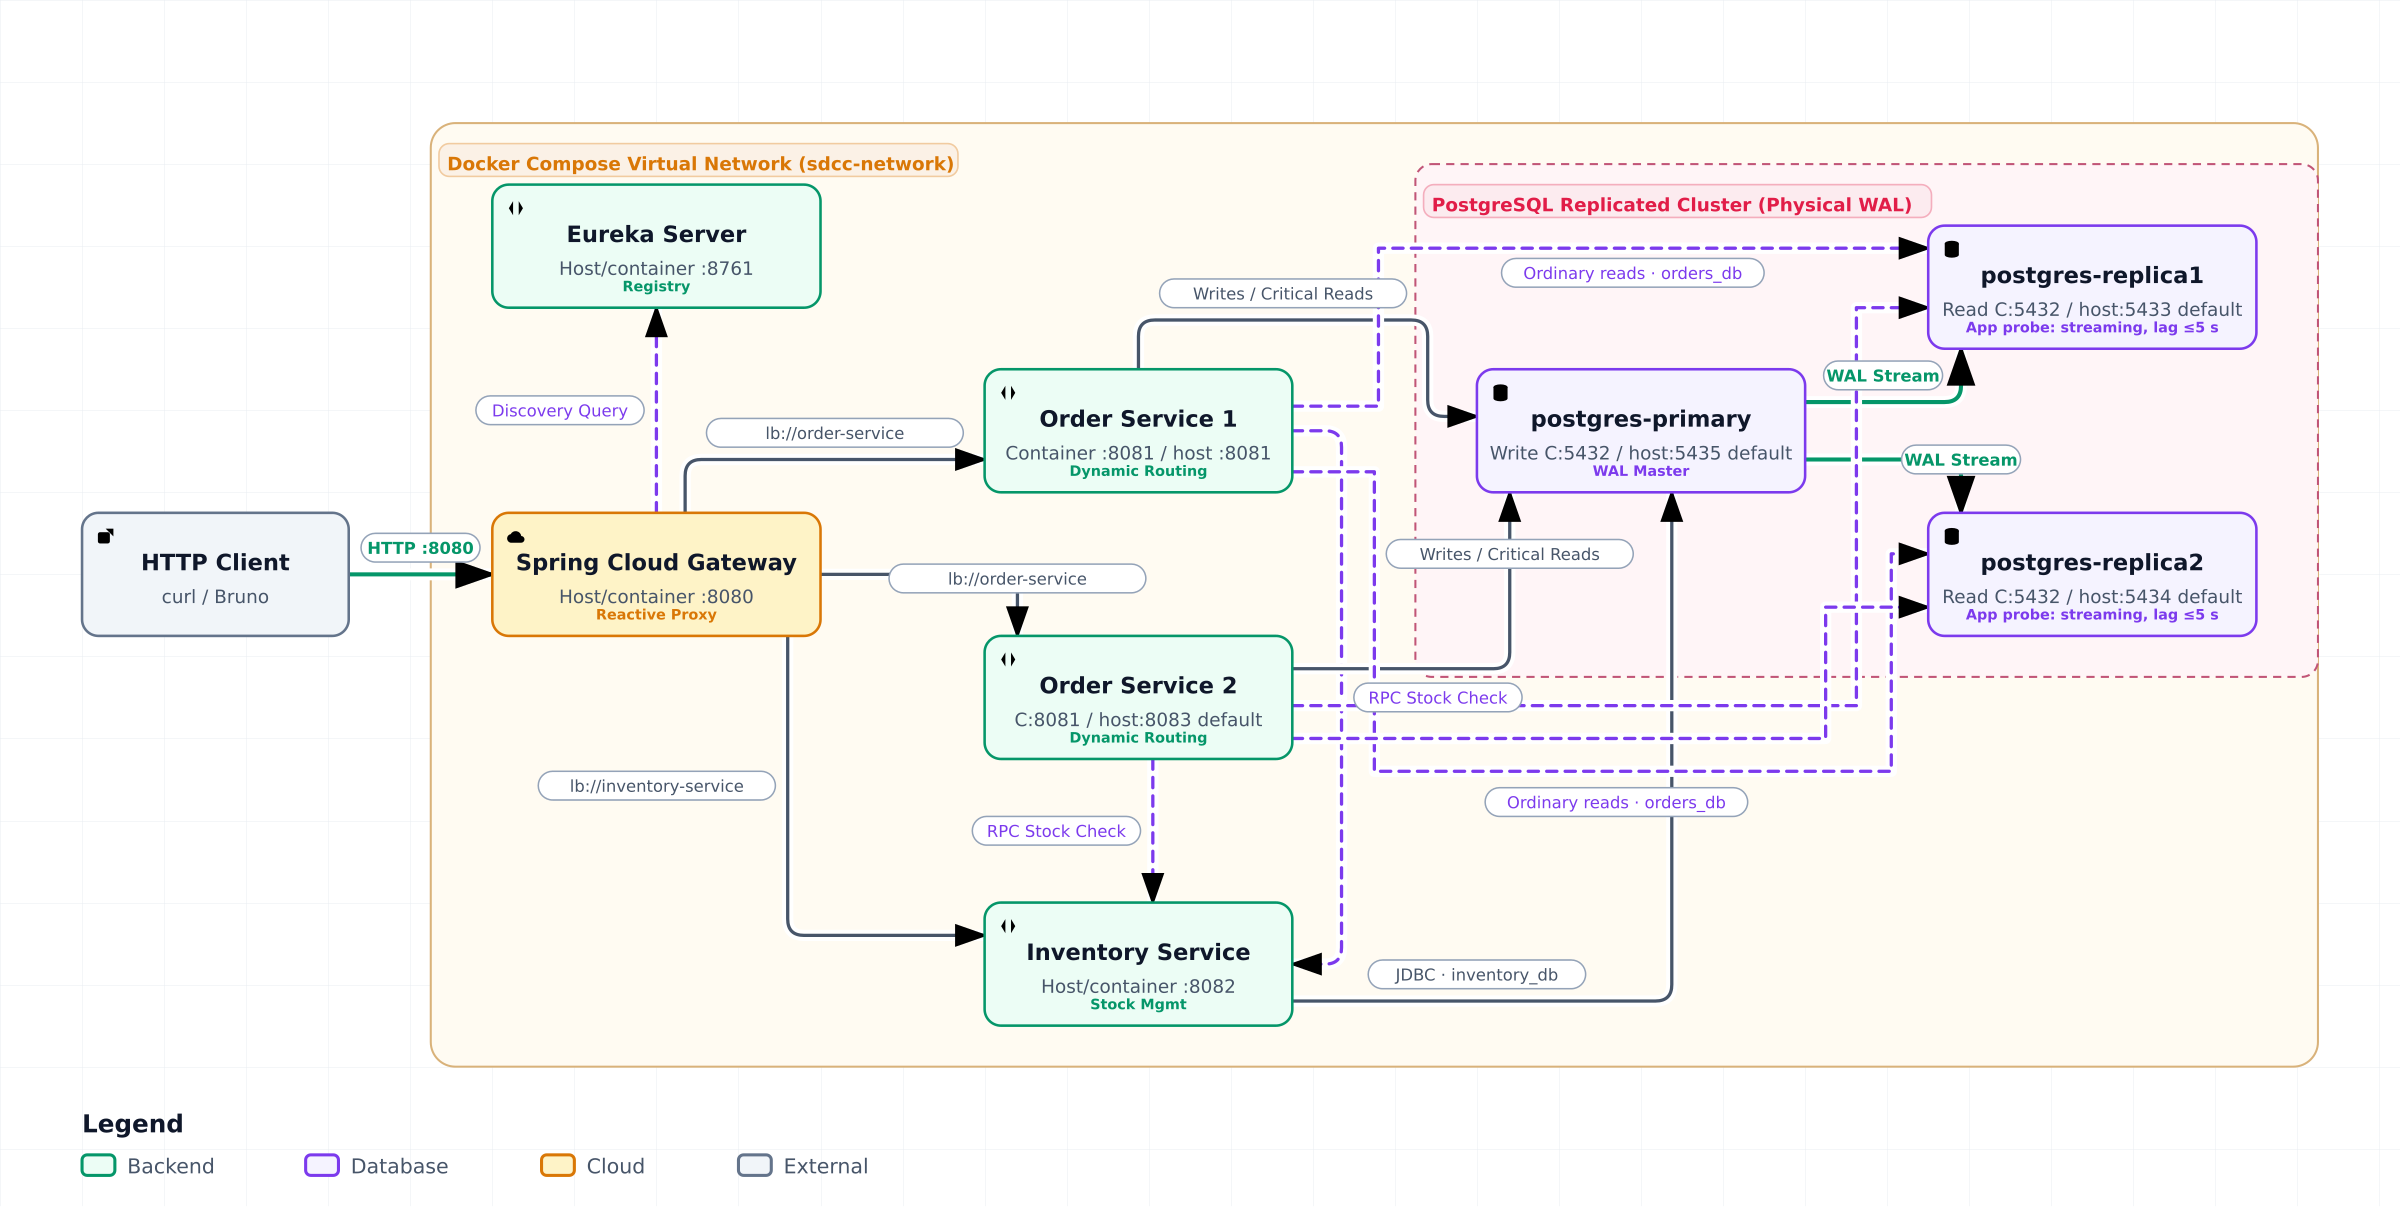
\includegraphics[width=\textwidth]{architecture_light.png}
  \caption{Topología del Clúster: Gateway, Microservicios (Eureka/LoadBalancer) y Persistencia PostgreSQL Replicada (Primary y Replicas WAL).}
  \label{fig:arquitectura}
\end{figure}

\vspace{0.5em}
\noindent
Para interactuar con la versión dinámica vectorial, consulte el \href{https://github.com/yan2005dris-afk/SDCC---microservices-with-gateway-and-loadbalancer/blob/70ee0a32947f29515b9d0ab2961b1314c0b0938c/docs/architecture/architecture.html}{Diagrama interactivo de la arquitectura en HTML}.

\section{Identificación y alcance}\label{identificaciuxf3n-y-alcance}

\begin{itemize}
\tightlist
\item
  \textbf{Fecha del entorno:} 2026-11-24, hora local UTC−05:00.
\item
  \textbf{Commit base del checkout:} \texttt{a431612}.
\item
  \textbf{Stack:} Docker Engine 29.10.0, Docker Compose 5.8.0,
  PostgreSQL 17; Bruno CLI 4.3.0.
\item
  \textbf{Stack de prueba:} proyecto Compose
  \texttt{sdcc-pdd-junie-test}; \texttt{compose.yaml} más
  \href{https://github.com/yan2005dris-afk/SDCC---microservices-with-gateway-and-loadbalancer/blob/70ee0a32947f29515b9d0ab2961b1314c0b0938c/docs/evidencias/compose-test-overlay.yaml}{\texttt{docs/\codebreak{}evide\codebreak{}ncias/\codebreak{}comp\codebreak{}ose-\codebreak{}test-\codebreak{}o\codebreak{}verlay.\codebreak{}yam\codebreak{}l}}.
  El puerto host 8083 estaba ocupado por otro proyecto, por lo que la
  segunda instancia se publicó temporalmente en 18083; su puerto interno
  y el registro Eureka no cambiaron. No se modificó Compose de
  producción.
\item
  \textbf{Datos y seguridad:} pedidos con nombres de demostración y
  correos \texttt{example.invalid}. Los anexos omiten cuerpos con datos
  de cliente y credenciales. Los pedidos de prueba se conservaron en el
  volumen; no se borraron volúmenes.
\item
  \textbf{Índice de salidas:}
  \href{https://github.com/yan2005dris-afk/SDCC---microservices-with-gateway-and-loadbalancer/blob/70ee0a32947f29515b9d0ab2961b1314c0b0938c/docs/evidencias/README.md}{docs/evidencias/README.md}.
\end{itemize}

\section{Resultados observados P01--P08}\label{resultados-observados-p01p08}

A continuación se sintetiza el comportamiento medido experimentalmente en cada uno de los ocho escenarios obligatorios:

\vspace{0.5em}
\begin{tcolorbox}[
  enhanced,
  colback=white,
  colframe=UPSEBlue,
  arc=2.5mm,
  boxrule=0.8pt,
  left=0pt,
  right=0pt,
  top=0pt,
  bottom=0pt,
  boxsep=0pt
]
\renewcommand{\arraystretch}{1.35}
\begin{tabularx}{\textwidth}{>{\bfseries\color{UPSEBlue}\centering\arraybackslash}p{22mm} >{\raggedright\arraybackslash}X}
\rowcolor{UPSEBlue}
\textcolor{white}{\textbf{Escenario}} & \textcolor{white}{\textbf{Resultado Experimental Medido en el Clúster}} \\
\midrule
\rowcolor{LightGrayBg}
P01 & \textbf{Descubrimiento Dinámico:} Eureka HTTP 200; \texttt{API-GATEWAY}, \texttt{INVENTORY-SERVICE} y las dos instancias \texttt{ORDER-SERVICE} en estado \texttt{UP}. Healthchecks sanos, cinco productos semilla en inventario y dos conexiones WAL activas (\texttt{streaming/async}). \\
P02 & \textbf{Balanceo de Carga HTTP:} En la primera ráfaga inmediatamente tras levantar Eureka, 100/100 respuestas fueron 503 porque el Gateway aún no consideraba listas las instancias (causa probable: ventana de health-check y caché de 5\,s; no medida, ver C03). Tras régimen estable, dos tandas de medición dieron \textbf{100/100 HTTP 200}, con distribución equitativa \textbf{50\% por instancia} y \textbf{50\% por réplica BD}. \\
\rowcolor{LightGrayBg}
P03 & \textbf{Tolerancia al Fallo de Instancia:} Antes, durante y después de detener \texttt{order-service-1}: 20/20, 80/80 y 20/20 HTTP 200, sin errores. Recuperación: \texttt{healthy} en 10,6\,s y primera respuesta de la instancia en 14,4\,s. \\
P04 & \textbf{Comunicación Inter-Servicio:} \texttt{POST /api/orders} válido devolvió 201 y enrutamiento a \texttt{PRIMARY} (ID 4 creado); el caso de stock insuficiente devolvió 400 Bad Request protegiendo la consistencia de inventario. \\
\rowcolor{LightGrayBg}
P05 & \textbf{Enrutamiento Read/Write Splitting:} Tres \texttt{GET} ordinarios devolvieron HTTP 200 distribuidos entre nodos \texttt{REPLICA\_2}, \texttt{REPLICA\_1}, \texttt{REPLICA\_1}. Las lecturas no tocaron el nodo primario. \\
P06 & \textbf{Fallo en Réplica de Lectura:} Con \texttt{postgres-replica1} detenida, 40/40 lecturas inmediatas HTTP 200; el selector la marcó \texttt{DOWN} en el primer fallo y reintentó en \texttt{REPLICA\_2} ($\sim$1\,s extra en una sola solicitud). Restaurada, volvió a \texttt{streaming/async}. \\
\rowcolor{LightGrayBg}
P07 & \textbf{Lectura Crítica Inmediata (Read-After-Write):} \texttt{GET /api/orders/4} con cabecera de consistencia crítica devolvió HTTP 200 directamente desde \texttt{PRIMARY}, lo que evita leer datos aún no replicados a las réplicas. \\
P08 & \textbf{Reincorporación en Caliente de Réplica:} Tras reactivar \texttt{postgres-replica1}, volvió a \texttt{streaming} WAL y la primera lectura servida por \texttt{REPLICA\_1} llegó \textbf{6,9\,s} después de arrancarla, sin reiniciar microservicios. \\
\bottomrule
\end{tabularx}
\end{tcolorbox}
\vspace{0.8em}

\section{Escenarios P01--P08 en detalle}\label{escenarios-detalle}

Para cada escenario se indican el objetivo, el procedimiento, el resultado
esperado, el resultado obtenido, la evidencia y el análisis. Las evidencias
de 2026-11-24 enlazan al commit evaluado; las repeticiones ampliadas de P03
y P06 (2026-11-25) están en \texttt{docs/evidencias/} y se generan con los
scripts de \texttt{scripts/experiments/}.

\subsection{P01 --- Descubrimiento dinámico}
\begin{itemize}
\tightlist
\item \textbf{Objetivo:} verificar que las instancias se registran en Eureka y se localizan por nombre lógico.
\item \textbf{Procedimiento:} \texttt{docker compose ps} del stack; \texttt{GET :8761/eureka/apps}; \texttt{GET :8080/actuator/health}; solicitudes funcionales vía Gateway (\texttt{lb://order-service}, \texttt{lb://inventory-service}).
\item \textbf{Resultado esperado:} \texttt{API-GATEWAY}, \texttt{INVENTORY-SERVICE} y dos instancias de \texttt{ORDER-SERVICE} en \texttt{UP}; el Gateway responde sin URLs fijas.
\item \textbf{Resultado obtenido:} Eureka HTTP 200 con \texttt{order-service-1:8081=UP}, \texttt{order-service-2:8083=UP}, \texttt{inventory-service:8082=UP} y \texttt{api-gateway:8080=UP}; Gateway 200; los 8 contenedores \texttt{healthy}; 5 productos semilla y 2 réplicas en \texttt{streaming/async}.
\item \textbf{Evidencia:} \evid{P01-discovery.log}.
\item \textbf{Análisis:} cada instancia se identifica por \texttt{host:puerto} en Eureka y por la cabecera \texttt{X-Instance-Id} en las respuestas; el Gateway y Orders resuelven a los servicios solo por su nombre lógico.
\end{itemize}

\subsection{P02 --- Balanceo HTTP}
\begin{itemize}
\tightlist
\item \textbf{Objetivo:} enviar al menos 100 solicitudes a un servicio con dos instancias y registrar cuál responde cada una.
\item \textbf{Procedimiento:} \texttt{scripts/experiments/test-p02-loadbalance.sh} (100 \texttt{GET /api/orders} vía Gateway, registra \texttt{X-Instance-Id} y \texttt{X-Database-Node}), tras confirmar un HTTP 200 desde cada instancia.
\item \textbf{Resultado esperado:} 100 respuestas exitosas repartidas entre ambas instancias por el LoadBalancer (round-robin).
\item \textbf{Resultado obtenido:} dos tandas de 100/100 HTTP 200; \texttt{order-service-1}=50 y \texttt{order-service-2}=50; \texttt{REPLICA\_1}=50 y \texttt{REPLICA\_2}=50; 0 errores HTTP o de transporte.
\item \textbf{Evidencia:} \evid{P02-loadbalance-startup-ready.log}, \evid{P02-loadbalance-stable.log}; diagnóstico de arranque en \evid{P02-loadbalance-startup.log} y \evid{P02-gateway-503.log}.
\item \textbf{Análisis:} el reparto exacto 50/50 confirma el round-robin de Spring Cloud LoadBalancer. Error transitorio observado: lanzada la ráfaga en cuanto Eureka mostró ambas instancias \texttt{UP}, el Gateway devolvió 100/100 HTTP 503 en 2--35\,ms (rechazo inmediato, no timeout). Causa probable: el LoadBalancer filtra instancias con un health-check propio (\texttt{/actuator/health/readiness}, intervalo y caché de 5\,s), así que \texttt{UP} en Eureka no implica disponibilidad inmediata en el Gateway. Por eso la medición válida exige antes un 200 desde cada instancia (C03--C05).
\end{itemize}

\subsection{P03 --- Fallo de instancia}
\begin{itemize}
\tightlist
\item \textbf{Objetivo:} detener una instancia de Orders y comprobar que el sistema sigue atendiendo mediante la otra; medir el tiempo de recuperación.
\item \textbf{Procedimiento:} \texttt{scripts/experiments/test-p03-instance-failover.sh} con \texttt{DURING=80}: 20 solicitudes antes; \texttt{docker stop order-service-1} en segundo plano y 80 solicitudes durante el apagado (una cada $\sim$0,27\,s); \texttt{docker start} midiendo el tiempo hasta \texttt{healthy} y hasta la primera respuesta servida por la instancia; 20 solicitudes después.
\item \textbf{Resultado esperado:} las solicitudes siguen respondiendo durante el fallo y la instancia vuelve a recibir tráfico tras recuperarse.
\item \textbf{Resultado obtenido:} antes 20/20 HTTP 200 (10/10 por instancia); durante 80/80 HTTP 200 (7 de \texttt{order-service-1} mientras terminaba su apagado ordenado y 73 de \texttt{order-service-2}); el apagado tardó 22,1\,s. Recuperación: contenedor \texttt{healthy} a los 10,6\,s y primera respuesta de \texttt{order-service-1} a los 14,4\,s del arranque; después 20/20 HTTP 200 (10/10).
\item \textbf{Evidencia:} \texttt{docs/evidencias/P03-instance-failover-full.log} (2026-11-25); ejecución previa en \evid{P03-order-failover.log}.
\item \textbf{Análisis:} no hubo errores porque la instancia se apaga ordenadamente (\texttt{timeout-per-shutdown-phase: 20s}): deja de registrarse en Eureka y termina las solicitudes en curso, y el Gateway reintenta los \texttt{GET} fallidos (hasta 2 veces ante 502/503 o errores de conexión). Una caída abrupta (\texttt{docker kill}) podría producir errores transitorios hasta que caduque la caché del LoadBalancer. Los $\sim$4\,s entre \texttt{healthy} y la primera respuesta corresponden al registro en Eureka y a la caché/health-check del Gateway.
\end{itemize}

\subsection{P04 --- Comunicación entre servicios}
\begin{itemize}
\tightlist
\item \textbf{Objetivo:} ejecutar una operación de negocio que requiera una llamada real de Orders a Inventory mediante descubrimiento dinámico.
\item \textbf{Procedimiento:} \texttt{POST /api/orders} vía Gateway con \texttt{X-Correlation-Id}: un pedido válido (2 unidades de \texttt{PROD-001}) y otro con 9999 unidades. Orders llama a \texttt{POST /api/inventory/reserve} con un \texttt{RestClient} \texttt{@LoadBalanced} sobre \texttt{http://inventory-service}.
\item \textbf{Resultado esperado:} 201 con stock reservado en el caso válido; rechazo controlado sin pedido confirmado en el caso sin stock.
\item \textbf{Resultado obtenido:} caso válido HTTP 201, pedido ID 4 en \texttt{PRIMARY} con estado \texttt{CONFIRMED}; caso sin stock HTTP 400. El mismo CID aparece en los logs de Gateway, Orders e Inventory para ambos casos.
\item \textbf{Evidencia:} \evid{P04-P05-P07-orders.log}.
\item \textbf{Análisis:} la traza por CID demuestra la cadena Gateway $\rightarrow$ Orders $\rightarrow$ Inventory sin URLs fijas. Inventory valida el stock y Orders traduce el rechazo en un 400 sin escribir el pedido, por lo que la respuesta no lleva \texttt{X-Database-Node}.
\end{itemize}

\subsection{P05 --- Enrutamiento de base de datos}
\begin{itemize}
\tightlist
\item \textbf{Objetivo:} demostrar que las escrituras usan el primario y las consultas ordinarias se distribuyen entre las dos réplicas.
\item \textbf{Procedimiento:} el \texttt{POST} de P04 y tres \texttt{GET /api/orders} con CID propio; consulta SQL del pedido 4 en \texttt{orders\_db}; logs de aplicación con el nodo usado.
\item \textbf{Resultado esperado:} escrituras en \texttt{PRIMARY}; lecturas ordinarias alternadas entre \texttt{REPLICA\_1} y \texttt{REPLICA\_2}.
\item \textbf{Resultado obtenido:} \texttt{POST} en \texttt{PRIMARY}; lecturas en \texttt{REPLICA\_2}, \texttt{REPLICA\_1} y \texttt{REPLICA\_1}, cada una con su CID en el log (\texttt{db=REPLICA\_n}); el pedido 4 es visible por SQL. En las 200 lecturas de P02 el reparto fue 50/50 entre réplicas.
\item \textbf{Evidencia:} \evid{P04-P05-P07-orders.log}, \evid{P02-loadbalance-stable.log}.
\item \textbf{Análisis:} el enrutamiento lo hace \texttt{DynamicRoutingDataSource} (\texttt{AbstractRoutingDataSource}) y la política está en \texttt{HealthAwareReplicaSelector}: round-robin entre las réplicas aptas. Cada instancia de Orders tiene su propio contador, por eso tres lecturas aisladas pueden repetir réplica; la distribución se aprecia en muestras grandes como P02.
\end{itemize}

\subsection{P06 --- Fallo de réplica PostgreSQL}
\begin{itemize}
\tightlist
\item \textbf{Objetivo:} detener una réplica y comprobar que las consultas continúan mediante la restante.
\item \textbf{Procedimiento:} \texttt{scripts/experiments/test-p06-replica-failover.sh}: estado de contenedores; 10 lecturas antes; \texttt{docker stop postgres-replica1} en segundo plano y 40 lecturas inmediatas; logs \texttt{db.route} y \texttt{replica.state} de ambas instancias de Orders; restauración.
\item \textbf{Resultado esperado:} lecturas sin interrupción servidas por \texttt{REPLICA\_2}; el selector retira a \texttt{REPLICA\_1} de la rotación.
\item \textbf{Resultado obtenido:} antes 10/10 HTTP 200 (5 por réplica); durante 40/40 HTTP 200, la primera aún en \texttt{REPLICA\_1} (27\,ms tras la orden de parada) y las 39 siguientes en \texttt{REPLICA\_2}. Logs: \texttt{attempt=1 result=FAILED} sobre \texttt{REPLICA\_1} (1003\,ms), \texttt{replica.state from=UP to=DOWN} y \texttt{replica.rotation action=LEAVE} en ambas instancias; la solicitud afectada tardó $\sim$1\,s más y respondió 200. Réplica de nuevo \texttt{healthy} a los 5,3\,s del arranque.
\item \textbf{Evidencia:} \texttt{docs/evidencias/P06-replica-failover-full.log} (2026-11-25); ejecución previa en \evid{P06-replica-failover.log}.
\item \textbf{Análisis:} la caída se detecta por dos vías: el sondeo periódico (cada 2\,s, timeout 1\,s) y el fallo de una solicitud real, que marca la réplica \texttt{DOWN} y reintenta en otra. El coste observado es una latencia extra de $\sim$1\,s en la primera solicitud afectada, sin errores para el cliente. Si fallaran ambas réplicas, la lectura se sirve desde el primario (\texttt{fallback-to-primary: true}).
\end{itemize}

\subsection{P07 --- Consistencia de lectura}
\begin{itemize}
\tightlist
\item \textbf{Objetivo:} crear un registro y consultarlo de inmediato con una operación crítica dirigida al primario.
\item \textbf{Procedimiento:} tras el \texttt{POST} de P04 (ID 4), \texttt{GET /api/orders/4} con \texttt{X-Consistency: critical} y CID propio.
\item \textbf{Resultado esperado:} HTTP 200 con el pedido recién creado, servido por \texttt{PRIMARY}.
\item \textbf{Resultado obtenido:} HTTP 200, mismo ID 4, \texttt{X-Database-Node: PRIMARY}; el CID aparece en el log con \texttt{db=PRIMARY}.
\item \textbf{Evidencia:} \evid{P04-P05-P07-orders.log}.
\item \textbf{Análisis:} la replicación es asíncrona, así que una réplica puede no tener aún el registro recién escrito. La política \emph{read-your-writes} envía las lecturas marcadas como críticas al primario y deja las ordinarias en las réplicas, para no cargar el primario con todas las lecturas.
\end{itemize}

\subsection{P08 --- Recuperación de réplica}
\begin{itemize}
\tightlist
\item \textbf{Objetivo:} reiniciar la réplica detenida, comprobar su recuperación y que vuelve a atender consultas.
\item \textbf{Procedimiento:} \texttt{docker start postgres-replica1} midiendo el tiempo; \texttt{pg\_stat\_replication} en el primario; \texttt{GET /api/orders} repetidos hasta recibir \texttt{X-Database-Node: REPLICA\_1}.
\item \textbf{Resultado esperado:} la réplica vuelve a \texttt{streaming} y reingresa a la rotación solo cuando es apta.
\item \textbf{Resultado obtenido:} contenedor \texttt{healthy}; dos réplicas \texttt{streaming/async} en el primario; primera lectura servida por \texttt{REPLICA\_1} 6,9\,s después del arranque, sin reiniciar microservicios.
\item \textbf{Evidencia:} \evid{P08-replica-rejoin.log}.
\item \textbf{Análisis:} una réplica es apta si está en recuperación, en \texttt{streaming} y con lag $\le$ 5\,s; reingresa tras 2 sondeos consecutivos correctos (\texttt{rejoin-threshold}). Esto explica los $\sim$7\,s: arranque de PostgreSQL, reconexión WAL y dos sondeos de 2\,s.
\end{itemize}

\section{Registro de verificaciones}\label{registro-de-verificaciones}

Cada verificación (C01--C21) indica qué se comprobó, cómo se hizo y su
resultado. \texttt{passed}: cumplió lo esperado; \texttt{failed}: no
cumplió; \texttt{not\_run}: no se ejecutó. \emph{Specs} remite a los
criterios S1, S2, \ldots{} definidos en \texttt{pdd/tasks/<nombre>.md};
\emph{Requerido} indica si la verificación es obligatoria para la entrega.
Los comandos completos están en cada archivo de evidencia enlazado.

\subsection{C01 --- Reproducibilidad, puertos y sintaxis del
script}\label{c01-reproducibilidad-puertos-y-sintaxis-del-script}

\begin{itemize}
\tightlist
\item
  \textbf{Specs:} \texttt{reproducib\codebreak{}ilidad-\codebreak{}ent\codebreak{}rega/\codebreak{}S1–S3},
  \texttt{coleccione\codebreak{}s-\codebreak{}medicion\codebreak{}/\codebreak{}S2}.
\item
  \textbf{Requerido:} sí.
\item
  \textbf{Comando exacto:}
  \texttt{docker\ \codebreak{}com\codebreak{}pose\ \codebreak{}-\codebreak{}p\ \codebreak{}sd\codebreak{}cc-\codebreak{}pdd-\codebreak{}jun\codebreak{}ie-\codebreak{}test\ \codebreak{}-\codebreak{}f\codebreak{}\ \codebreak{}compose.\codebreak{}y\codebreak{}aml\ \codebreak{}-\codebreak{}f\ \codebreak{}doc\codebreak{}s/\codebreak{}evidenci\codebreak{}as/\codebreak{}compose\codebreak{}-\codebreak{}test-\codebreak{}over\codebreak{}lay.\codebreak{}yaml\ \codebreak{}-\codebreak{}\/-\codebreak{}env-\codebreak{}file\codebreak{}\ \codebreak{}.\codebreak{}env.\codebreak{}exam\codebreak{}ple\ \codebreak{}config\codebreak{}\ \codebreak{}-\codebreak{}q};
  \texttt{bash\ \codebreak{}-\codebreak{}n\ \codebreak{}sc\codebreak{}ripts/\codebreak{}expe\codebreak{}riments/\codebreak{}te\codebreak{}st-\codebreak{}p02-\codebreak{}loa\codebreak{}dbalance.\codebreak{}s\codebreak{}h};
  \texttt{git\ diff\ -\/-check}.
\item
  \textbf{Código de salida:} 0 en los tres comandos.
\item
  \textbf{Salida observada:} Compose aceptó la configuración y el
  overlay; Bash y el diff no reportaron errores.
\item
  \textbf{Salida:} validación local (sin archivo de salida).
\item
  \textbf{Estado:} \textcolor{PassGreen}{\textbf{passed}}.
\end{itemize}

\subsection{C02 --- P01, descubrimiento y estado
base}\label{c02-p01-descubrimiento-y-estado-base}

\begin{itemize}
\tightlist
\item
  \textbf{Specs:} \texttt{informe-\codebreak{}ex\codebreak{}perimental\codebreak{}/\codebreak{}S1}.
\item
  \textbf{Requerido:} sí.
\item
  \textbf{Cómo se ejecutó:} \texttt{docker compose ps} del stack de prueba, consulta a Eureka (\texttt{GET :8761/eureka/apps}), y consultas \texttt{psql} a \texttt{inventory\_db} y \texttt{pg\_stat\_replication} en el primario.
\item
  \textbf{Código de salida:} 0; Eureka 200, Gateway 200 y componentes
  saludables.
\item
  \textbf{Salida observada:} tres aplicaciones registradas; dos Orders
  \texttt{UP}; cinco productos; dos conexiones WAL
  \texttt{streaming/async}.
\item
  \textbf{Salida:}
  \href{https://github.com/yan2005dris-afk/SDCC---microservices-with-gateway-and-loadbalancer/blob/70ee0a32947f29515b9d0ab2961b1314c0b0938c/docs/evidencias/P01-discovery.log}{P01-discovery.log}.
\item
  \textbf{Estado:} \textcolor{PassGreen}{\textbf{passed}}.
\end{itemize}

\subsection{\texorpdfstring{C03 --- P02, diagnóstico inmediato tras
Eureka
\texttt{UP}}{C03 --- P02, diagnóstico inmediato tras Eureka UP}}\label{c03-p02-diagnuxf3stico-inmediato-tras-eureka-up}

\begin{itemize}
\tightlist
\item
  \textbf{Specs:} \texttt{informe-\codebreak{}ex\codebreak{}perimental\codebreak{}/\codebreak{}S2}.
\item
  \textbf{Requerido:} no (diagnóstico de readiness anterior a la muestra
  válida).
\item
  \textbf{Cómo se ejecutó:} se detuvieron y relanzaron \texttt{order-service-1} y \texttt{order-service-2} (\texttt{docker compose stop} y \texttt{up -{}-wait}) y, en cuanto Eureka los mostró \texttt{UP}, se ejecutó \texttt{scripts/experiments/test-p02-loadbalance.sh} sin esperar a que el Gateway respondiera 200.
\item
  \textbf{Código de salida del script:} 1.
\item
  \textbf{Salida observada:} Eureka ya mostraba ambos \texttt{UP}, pero
  100/100 HTTP 503; 100 errores HTTP y 100 solicitudes sin las dos
  cabeceras de ruta; 0 errores de transporte. La evidencia no determina
  por sí sola la causa interna de esa ventana.
\item
  \textbf{Salida:}
  \href{https://github.com/yan2005dris-afk/SDCC---microservices-with-gateway-and-loadbalancer/blob/70ee0a32947f29515b9d0ab2961b1314c0b0938c/docs/evidencias/P02-loadbalance-startup.log}{P02-loadbalance-startup.log}
  y
  \href{https://github.com/yan2005dris-afk/SDCC---microservices-with-gateway-and-loadbalancer/blob/70ee0a32947f29515b9d0ab2961b1314c0b0938c/docs/evidencias/P02-gateway-503.log}{P02-gateway-503.log}
  (100 líneas \texttt{503\ \codebreak{}SERVIC\codebreak{}E\_UNAVAILA\codebreak{}BLE}).
\item
  \textbf{Resultado esperado:} sí. Es un diagnóstico de la ventana de arranque y no invalida P02 (ver C04 y C05).
\item
  \textbf{Estado:} \textcolor{FailRed}{\textbf{failed}}.
\end{itemize}

\subsection{C04 --- P02, muestra después de readiness de
Gateway}\label{c04-p02-muestra-despuuxe9s-de-readiness-de-gateway}

\begin{itemize}
\tightlist
\item
  \textbf{Specs:} \texttt{coleccione\codebreak{}s-\codebreak{}medicion\codebreak{}/\codebreak{}S2},
  \texttt{informe-\codebreak{}ex\codebreak{}perimental\codebreak{}/\codebreak{}S2}.
\item
  \textbf{Requerido:} sí.
\item
  \textbf{Comando exacto:}
  \texttt{curl\ \codebreak{}-\codebreak{}\/-\codebreak{}si\codebreak{}lent\ \codebreak{}-\codebreak{}\/-\codebreak{}sh\codebreak{}ow-\codebreak{}error\ \codebreak{}-\codebreak{}\/-\codebreak{}dump-\codebreak{}hea\codebreak{}der\ \codebreak{}-\codebreak{}\ \codebreak{}-\codebreak{}\/-\codebreak{}o\codebreak{}utput\ \codebreak{}/\codebreak{}dev\codebreak{}/\codebreak{}null\ \codebreak{}-\codebreak{}\/-\codebreak{}c\codebreak{}onnect-\codebreak{}tim\codebreak{}eout\ \codebreak{}3\ \codebreak{}-\codebreak{}\/-\codebreak{}max-\codebreak{}time\ \codebreak{}1\codebreak{}0\ \codebreak{}-\codebreak{}\/-\codebreak{}write\codebreak{}-\codebreak{}out\ \codebreak{}\$\textquotesingle{}\textbackslash{}n\%\codebreak{}\{http\_code\codebreak{}\}\textquotesingle{}\ \codebreak{}http:/\codebreak{}/\codebreak{}localhost:\codebreak{}8080/\codebreak{}api/\codebreak{}o\codebreak{}rders}
  repetido hasta observar HTTP 200 desde \texttt{order-service-1} y
  \texttt{order-service-2}; después
  \texttt{bash\ \codebreak{}scrip\codebreak{}ts/\codebreak{}experim\codebreak{}ents/\codebreak{}test-\codebreak{}p02-\codebreak{}loadba\codebreak{}lance.\codebreak{}sh}.
\item
  \textbf{Código de salida:} 0.
\item
  \textbf{Salida observada:} 100/100 HTTP 200,
  \texttt{order-service-1=50}, \texttt{order-service-2=50},
  \texttt{REPLICA\_1=50}, \texttt{REPLICA\_2=50}, cero errores HTTP,
  transporte o cabeceras; reconciliación 100/100.
\item
  \textbf{Salida:}
  \href{https://github.com/yan2005dris-afk/SDCC---microservices-with-gateway-and-loadbalancer/blob/70ee0a32947f29515b9d0ab2961b1314c0b0938c/docs/evidencias/P02-loadbalance-startup-ready.log}{P02-loadbalance-startup-ready.log}.
\item
  \textbf{Estado:} \textcolor{PassGreen}{\textbf{passed}}.
\end{itemize}

\subsection{C05 --- P02, régimen
estable}\label{c05-p02-ruxe9gimen-estable}

\begin{itemize}
\tightlist
\item
  \textbf{Specs:} \texttt{coleccione\codebreak{}s-\codebreak{}medicion\codebreak{}/\codebreak{}S2},
  \texttt{informe-\codebreak{}ex\codebreak{}perimental\codebreak{}/\codebreak{}S2}.
\item
  \textbf{Requerido:} sí.
\item
  \textbf{Comando exacto:}
  \texttt{sleep\ \codebreak{}15\ \codebreak{}\&\codebreak{}\&\ \codebreak{}bash\ \codebreak{}scr\codebreak{}ipts/\codebreak{}exper\codebreak{}iments/\codebreak{}tes\codebreak{}t-\codebreak{}p02-\codebreak{}load\codebreak{}balance.\codebreak{}sh}.
\item
  \textbf{Código de salida:} 0.
\item
  \textbf{Salida observada:} 100/100 HTTP 200, 50/50 por instancia y
  50/50 por réplica, cero errores; reconciliación 100/100.
\item
  \textbf{Salida:}
  \href{https://github.com/yan2005dris-afk/SDCC---microservices-with-gateway-and-loadbalancer/blob/70ee0a32947f29515b9d0ab2961b1314c0b0938c/docs/evidencias/P02-loadbalance-stable.log}{P02-loadbalance-stable.log}.
\item
  \textbf{Estado:} \textcolor{PassGreen}{\textbf{passed}}.
\end{itemize}

\subsection{C06 --- P02, contabilización de fallos de
transporte}\label{c06-p02-contabilizaciuxf3n-de-fallos-de-transporte}

\begin{itemize}
\tightlist
\item
  \textbf{Specs:} \texttt{coleccione\codebreak{}s-\codebreak{}medicion\codebreak{}/\codebreak{}S2}.
\item
  \textbf{Requerido:} sí.
\item
  \textbf{Comando exacto:}
  \texttt{GATEWAY\_UR\codebreak{}L=\codebreak{}http:/\codebreak{}/\codebreak{}1\codebreak{}27.\codebreak{}0.\codebreak{}0.\codebreak{}1:1\codebreak{}\ \codebreak{}TOTAL\_REQ\codebreak{}UESTS=\codebreak{}100\ \codebreak{}bash\ \codebreak{}scrip\codebreak{}ts/\codebreak{}experim\codebreak{}ents/\codebreak{}test-\codebreak{}p02-\codebreak{}loadba\codebreak{}lance.\codebreak{}sh}.
\item
  \textbf{Código de salida del script:} 1 (esperado para respuestas
  fallidas).
\item
  \textbf{Salida observada:} 100 intentos, 100 fallos curl 7, estado
  HTTP 000, cero respuestas HTTP, 100 errores de transporte y
  reconciliación 100/100; el wrapper de comprobación terminó en 0 al
  verificar la salida esperada.
\item
  \textbf{Salida:}
  \href{https://github.com/yan2005dris-afk/SDCC---microservices-with-gateway-and-loadbalancer/blob/70ee0a32947f29515b9d0ab2961b1314c0b0938c/docs/evidencias/P02-fault-injection.log}{P02-fault-injection.log}.
\item
  \textbf{Estado:} \textcolor{PassGreen}{\textbf{passed}}.
\end{itemize}

\subsection{C07 --- P02, límite mínimo de
solicitudes}\label{c07-p02-luxedmite-muxednimo-de-solicitudes}

\begin{itemize}
\tightlist
\item
  \textbf{Specs:} \texttt{coleccione\codebreak{}s-\codebreak{}medicion\codebreak{}/\codebreak{}S2}.
\item
  \textbf{Requerido:} no (caso de borde adicional).
\item
  \textbf{Comando exacto:}
  \texttt{TOTAL\_REQU\codebreak{}ESTS=\codebreak{}99\ \codebreak{}ba\codebreak{}sh\ \codebreak{}scripts\codebreak{}/\codebreak{}experimen\codebreak{}ts/\codebreak{}test-\codebreak{}p0\codebreak{}2-\codebreak{}loadbala\codebreak{}nce.\codebreak{}sh}.
\item
  \textbf{Código de salida:} 2 (esperado).
\item
  \textbf{Salida observada:} el script rechazó explícitamente un valor
  menor que 100 antes de enviar solicitudes.
\item
  \textbf{Salida:} terminal local (sin archivo).
\item
  \textbf{Estado:} \textcolor{PassGreen}{\textbf{passed}}.
\end{itemize}

\subsection{C08 --- Colección Bruno, creación, encadenamiento y
rechazo}\label{c08-colecciuxf3n-bruno-creaciuxf3n-encadenamiento-y-rechazo}

\begin{itemize}
\tightlist
\item
  \textbf{Specs:} \texttt{coleccione\codebreak{}s-\codebreak{}medicion\codebreak{}/\codebreak{}S1},
  \texttt{coleccione\codebreak{}s-\codebreak{}medicion\codebreak{}/\codebreak{}S3}.
\item
  \textbf{Requerido:} sí.
\item
  \textbf{Comando exacto:}
  \texttt{cd\ \codebreak{}tests/\codebreak{}b\codebreak{}runo/\codebreak{}colle\codebreak{}ction\ \codebreak{}\&\&\ \codebreak{}b\codebreak{}ru\ \codebreak{}run\ \codebreak{}-\codebreak{}r\ \codebreak{}-\codebreak{}\/-\codebreak{}env\ \codebreak{}loc\codebreak{}al\ \codebreak{}-\codebreak{}\/-\codebreak{}repo\codebreak{}rter-\codebreak{}json\ \codebreak{}.\codebreak{}.\codebreak{}/\codebreak{}.\codebreak{}.\codebreak{}/\codebreak{}.\codebreak{}.\codebreak{}/\codebreak{}d\codebreak{}ocs/\codebreak{}eviden\codebreak{}cias/\codebreak{}Bruno\codebreak{}-\codebreak{}collectio\codebreak{}n-\codebreak{}results.\codebreak{}json\ \codebreak{}-\codebreak{}\/-\codebreak{}re\codebreak{}porter-\codebreak{}ski\codebreak{}p-\codebreak{}body\ \codebreak{}-\codebreak{}\/-\codebreak{}reporter-\codebreak{}s\codebreak{}kip-\codebreak{}all-\codebreak{}he\codebreak{}aders}.
\item
  \textbf{Código de salida:} 0.
\item
  \textbf{Salida observada:} 6/6 solicitudes y 13/13 aserciones; POST
  201, ID dinámico reutilizado por lectura crítica 200 en PRIMARY,
  consulta de inventario 200 y rechazo por stock 400. El reporte JSON
  omite cuerpos y cabeceras.
\item
  \textbf{Salida:}
  \href{https://github.com/yan2005dris-afk/SDCC---microservices-with-gateway-and-loadbalancer/blob/70ee0a32947f29515b9d0ab2961b1314c0b0938c/docs/evidencias/Bruno-collection-results.json}{Bruno-collection-results.json}.
\item
  \textbf{Estado:} \textcolor{PassGreen}{\textbf{passed}}.
\end{itemize}

\subsection{C09 --- Ejecución del archivo HTTP Client de
JetBrains}\label{c09-ejecuciuxf3n-del-archivo-http-client-de-jetbrains}

\begin{itemize}
\tightlist
\item
  \textbf{Specs:} \texttt{coleccione\codebreak{}s-\codebreak{}medicion\codebreak{}/\codebreak{}S1},
  \texttt{coleccione\codebreak{}s-\codebreak{}medicion\codebreak{}/\codebreak{}S3}.
\item
  \textbf{Requerido:} sí.
\item
  \textbf{Comando exacto:} \texttt{docker\ run\ -{}-rm\ -{}-network\ host\ -v\ "\$PWD/tests/http:/workdir"\ -v\ /tmp/ij:/report\ jetbrains/intellij-http-client\ -{}-report=/report\ api-tests.http}
  (imagen oficial de la CLI \texttt{ijhttp}, contra el stack de pruebas
  levantado con el overlay de Compose). Ejecutado el 2026-11-25, un día
  después del resto de mediciones.
\item
  \textbf{Resultado observado:} 12 solicitudes completadas, 0 con pruebas
  fallidas (\texttt{RUN SUCCESSFUL}). El informe XML reporta 24 casos,
  0 fallos, 0 errores y 0 omitidos. Esto incluye el encadenamiento
  \texttt{client.\codebreak{}glo\codebreak{}bal.\codebreak{}set("o\codebreak{}rderId",\codebreak{}\ \codebreak{}r\codebreak{}esponse.\codebreak{}bo\codebreak{}dy.\codebreak{}id)}
  del \texttt{POST} de pedido.
\item
  \textbf{Salida:} \texttt{docs/\codebreak{}evidencias/\codebreak{}C09-\codebreak{}ijhttp.\codebreak{}log}
  (local; aún sin publicar en el commit evaluado).
\item
  \textbf{Estado:} \textcolor{PassGreen}{\textbf{passed}}.
\end{itemize}

\subsection{C10 --- P03, caída de
instancia}\label{c10-p03-cauxedda-de-instancia}

\begin{itemize}
\tightlist
\item
  \textbf{Specs:} \texttt{informe-\codebreak{}ex\codebreak{}perimental\codebreak{}/\codebreak{}S3}.
\item
  \textbf{Requerido:} sí.
\item
  \textbf{Cómo se ejecutó:} \texttt{docker stop order-service-1}; 20 \texttt{GET /api/orders} inmediatos y 20 más tras 4\,s vía Gateway con \texttt{curl}; luego \texttt{docker start order-service-1}.
\item
  \textbf{Código de salida:} 0, incluyendo la comprobación de
  restauración.
\item
  \textbf{Salida observada:} 40/40 HTTP 200 solo desde
  \texttt{order-service-2}; componente restaurado \texttt{healthy},
  Eureka \texttt{UP}.
\item
  \textbf{Salida:}
  \href{https://github.com/yan2005dris-afk/SDCC---microservices-with-gateway-and-loadbalancer/blob/70ee0a32947f29515b9d0ab2961b1314c0b0938c/docs/evidencias/P03-order-failover.log}{P03-order-failover.log}.
\item
  \textbf{Repetición ampliada (2026-11-25):} con fases antes, durante y después y tiempo de recuperación; ver P03 en la sección~\ref{escenarios-detalle}.
\item
  \textbf{Estado:} \textcolor{PassGreen}{\textbf{passed}}.
\end{itemize}

\subsection{C11 --- P04, pedido válido y reserva entre
servicios}\label{c11-p04-pedido-vuxe1lido-y-reserva-entre-servicios}

\begin{itemize}
\tightlist
\item
  \textbf{Specs:} \texttt{informe-\codebreak{}ex\codebreak{}perimental\codebreak{}/\codebreak{}S1},
  \texttt{informe-\codebreak{}ex\codebreak{}perimental\codebreak{}/\codebreak{}S2}.
\item
  \textbf{Requerido:} sí.
\item
  \textbf{Comando exacto:}
  \texttt{curl\ \codebreak{}-\codebreak{}\/-\codebreak{}si\codebreak{}lent\ \codebreak{}-\codebreak{}\/-\codebreak{}sh\codebreak{}ow-\codebreak{}error\ \codebreak{}-\codebreak{}\/-\codebreak{}include\ \codebreak{}-\codebreak{}\/-\codebreak{}request\codebreak{}\ \codebreak{}POST\ \codebreak{}-\codebreak{}\/-\codebreak{}h\codebreak{}eader\ \codebreak{}\textquotesingle{}Con\codebreak{}tent-\codebreak{}Type:\codebreak{}\ \codebreak{}applicati\codebreak{}on/\codebreak{}json\textquotesingle{}\ \codebreak{}-\codebreak{}\/-\codebreak{}header\ \codebreak{}\textquotesingle{}\codebreak{}X-\codebreak{}Correlat\codebreak{}ion-\codebreak{}Id:\ \codebreak{}sd\codebreak{}cc-\codebreak{}p04-\codebreak{}evi\codebreak{}dence-\codebreak{}orde\codebreak{}r-\codebreak{}01\textquotesingle{}\ \codebreak{}-\codebreak{}\/-\codebreak{}d\codebreak{}ata\ \codebreak{}\textquotesingle{}\{"cus\codebreak{}tomerName"\codebreak{}:"Cliente\ \codebreak{}Demo",\codebreak{}"cus\codebreak{}tomerEmail\codebreak{}":"demo@ex\codebreak{}ample.\codebreak{}inva\codebreak{}lid",\codebreak{}"prod\codebreak{}uctCode":"\codebreak{}PROD-\codebreak{}001",\codebreak{}"quantity"\codebreak{}:2,\codebreak{}"unitPr\codebreak{}ice":1899.\codebreak{}99\}\textquotesingle{}\ \codebreak{}http:\codebreak{}/\codebreak{}/\codebreak{}localhos\codebreak{}t:8080/\codebreak{}api\codebreak{}/\codebreak{}orders}.
\item
  \textbf{Resultado reportado:} 201, ID real 4,
  \texttt{X-\codebreak{}Database\codebreak{}-\codebreak{}Node:\ \codebreak{}PRI\codebreak{}MARY}; SQL \texttt{orders} muestra estado
  \texttt{CONFIRMED}. Logs enlazan Gateway, Order e Inventory por CID.
\item
  \textbf{Salida:}
  \href{https://github.com/yan2005dris-afk/SDCC---microservices-with-gateway-and-loadbalancer/blob/70ee0a32947f29515b9d0ab2961b1314c0b0938c/docs/evidencias/P04-P05-P07-orders.log}{P04-P05-P07-orders.log}.
\item
  \textbf{Estado:} \textcolor{PassGreen}{\textbf{passed}}.
\end{itemize}

\subsection{C12 --- P04, stock
insuficiente}\label{c12-p04-stock-insuficiente}

\begin{itemize}
\tightlist
\item
  \textbf{Specs:} \texttt{informe-\codebreak{}ex\codebreak{}perimental\codebreak{}/\codebreak{}S1},
  \texttt{informe-\codebreak{}ex\codebreak{}perimental\codebreak{}/\codebreak{}S2}.
\item
  \textbf{Requerido:} sí.
\item
  \textbf{Comando exacto:}
  \texttt{curl\ \codebreak{}-\codebreak{}\/-\codebreak{}si\codebreak{}lent\ \codebreak{}-\codebreak{}\/-\codebreak{}sh\codebreak{}ow-\codebreak{}error\ \codebreak{}-\codebreak{}\/-\codebreak{}include\ \codebreak{}-\codebreak{}\/-\codebreak{}request\codebreak{}\ \codebreak{}POST\ \codebreak{}-\codebreak{}\/-\codebreak{}h\codebreak{}eader\ \codebreak{}\textquotesingle{}Con\codebreak{}tent-\codebreak{}Type:\codebreak{}\ \codebreak{}applicati\codebreak{}on/\codebreak{}json\textquotesingle{}\ \codebreak{}-\codebreak{}\/-\codebreak{}header\ \codebreak{}\textquotesingle{}\codebreak{}X-\codebreak{}Correlat\codebreak{}ion-\codebreak{}Id:\ \codebreak{}sd\codebreak{}cc-\codebreak{}p04-\codebreak{}evi\codebreak{}dence-\codebreak{}reje\codebreak{}ct-\codebreak{}01\textquotesingle{}\ \codebreak{}-\codebreak{}\/-\codebreak{}data\ \codebreak{}\textquotesingle{}\{"cu\codebreak{}stomerName\codebreak{}":"Cliente\codebreak{}\ \codebreak{}Demo\ \codebreak{}Sin\ \codebreak{}Stock",\codebreak{}"cu\codebreak{}stomerEmai\codebreak{}l":"sin-\codebreak{}st\codebreak{}ock@exampl\codebreak{}e.\codebreak{}invalid"\codebreak{},\codebreak{}"productC\codebreak{}ode":"PROD\codebreak{}-\codebreak{}001",\codebreak{}"qua\codebreak{}ntity":999\codebreak{}9,\codebreak{}"unitPri\codebreak{}ce":1899.\codebreak{}9\codebreak{}9\}\textquotesingle{}\ \codebreak{}http:/\codebreak{}/\codebreak{}localhost\codebreak{}:8080/\codebreak{}api/\codebreak{}orders}.
\item
  \textbf{Resultado reportado:} HTTP 400; el Gateway y Order/Inventory
  registraron el CID. El rechazo no escribió en la base, por eso la
  respuesta no trae \texttt{X-Database-Node}.
\item
  \textbf{Salida:}
  \href{https://github.com/yan2005dris-afk/SDCC---microservices-with-gateway-and-loadbalancer/blob/70ee0a32947f29515b9d0ab2961b1314c0b0938c/docs/evidencias/P04-P05-P07-orders.log}{P04-P05-P07-orders.log}.
\item
  \textbf{Estado:} \textcolor{PassGreen}{\textbf{passed}}.
\end{itemize}

\subsection{C13 --- P05, lecturas ordinarias y
correlación}\label{c13-p05-lecturas-ordinarias-y-correlaciuxf3n}

\begin{itemize}
\tightlist
\item
  \textbf{Specs:} \texttt{informe-\codebreak{}ex\codebreak{}perimental\codebreak{}/\codebreak{}S1},
  \texttt{informe-\codebreak{}ex\codebreak{}perimental\codebreak{}/\codebreak{}S2}.
\item
  \textbf{Requerido:} sí.
\item
  \textbf{Comando exacto:}
  \texttt{for\ \codebreak{}cid\ \codebreak{}in\codebreak{}\ \codebreak{}sdcc-\codebreak{}p05-\codebreak{}evidence-\codebreak{}r\codebreak{}ead-\codebreak{}01\ \codebreak{}sdc\codebreak{}c-\codebreak{}p05-\codebreak{}evid\codebreak{}ence-\codebreak{}read-\codebreak{}02\ \codebreak{}sdcc-\codebreak{}p0\codebreak{}5-\codebreak{}evidence\codebreak{}-\codebreak{}read-\codebreak{}03;\codebreak{}\ \codebreak{}do\ \codebreak{}curl\ \codebreak{}-\codebreak{}\/\codebreak{}-\codebreak{}silent\ \codebreak{}-\codebreak{}\/\codebreak{}-\codebreak{}show-\codebreak{}erro\codebreak{}r\ \codebreak{}-\codebreak{}\/-\codebreak{}inclu\codebreak{}de\ \codebreak{}-\codebreak{}\/-\codebreak{}requ\codebreak{}est\ \codebreak{}GET\ \codebreak{}-\codebreak{}\/\codebreak{}-\codebreak{}header\ \codebreak{}\textquotesingle{}C\codebreak{}ontent-\codebreak{}Typ\codebreak{}e:\ \codebreak{}applica\codebreak{}tion/\codebreak{}json\textquotesingle{}\codebreak{}\ \codebreak{}-\codebreak{}\/-\codebreak{}header\codebreak{}\ \codebreak{}"X-\codebreak{}Correl\codebreak{}ation-\codebreak{}Id:\ \codebreak{}\$cid"\ \codebreak{}http\codebreak{}:/\codebreak{}/\codebreak{}localho\codebreak{}st:8080/\codebreak{}ap\codebreak{}i/\codebreak{}orders;\codebreak{}\ \codebreak{}done};
  consulta SQL del pedido 4 en \texttt{orders\_db}.
\item
  \textbf{Resultado reportado:} tres 200 desde \texttt{REPLICA\_2},
  \texttt{REPLICA\_1}, \texttt{REPLICA\_1}; los CIDs corresponden a logs
  de Gateway y Orders; cuatro pedidos visibles en esa muestra.
\item
  \textbf{Salida:}
  \href{https://github.com/yan2005dris-afk/SDCC---microservices-with-gateway-and-loadbalancer/blob/70ee0a32947f29515b9d0ab2961b1314c0b0938c/docs/evidencias/P04-P05-P07-orders.log}{P04-P05-P07-orders.log}.
\item
  \textbf{Estado:} \textcolor{PassGreen}{\textbf{passed}}.
\end{itemize}

\subsection{C14 --- P06, caída de
réplica}\label{c14-p06-cauxedda-de-ruxe9plica}

\begin{itemize}
\tightlist
\item
  \textbf{Specs:} \texttt{informe-\codebreak{}ex\codebreak{}perimental\codebreak{}/\codebreak{}S3}.
\item
  \textbf{Requerido:} sí.
\item
  \textbf{Cómo se ejecutó:} \texttt{docker stop postgres-replica1}; espera de 4\,s; 20 \texttt{GET /api/orders} vía Gateway con \texttt{curl}; luego \texttt{docker start postgres-replica1}.
\item
  \textbf{Código de salida:} 0, incluida la comprobación de
  restauración.
\item
  \textbf{Salida observada:} 20/20 HTTP 200 desde \texttt{REPLICA\_2};
  Compose \texttt{healthy} al restaurar y dos filas \texttt{streaming}
  en el primario.
\item
  \textbf{Salida:}
  \href{https://github.com/yan2005dris-afk/SDCC---microservices-with-gateway-and-loadbalancer/blob/70ee0a32947f29515b9d0ab2961b1314c0b0938c/docs/evidencias/P06-replica-failover.log}{P06-replica-failover.log}.
\item
  \textbf{Repetición ampliada (2026-11-25):} con lecturas inmediatas y logs del selector; ver P06 en la sección~\ref{escenarios-detalle}.
\item
  \textbf{Estado:} \textcolor{PassGreen}{\textbf{passed}}.
\end{itemize}

\subsection{C15 --- P07, lectura crítica por ID
real}\label{c15-p07-lectura-cruxedtica-por-id-real}

\begin{itemize}
\tightlist
\item
  \textbf{Specs:} \texttt{informe-\codebreak{}ex\codebreak{}perimental\codebreak{}/\codebreak{}S1},
  \texttt{informe-\codebreak{}ex\codebreak{}perimental\codebreak{}/\codebreak{}S2}.
\item
  \textbf{Requerido:} sí.
\item
  \textbf{Comando exacto:}
  \texttt{curl\ \codebreak{}-\codebreak{}\/-\codebreak{}si\codebreak{}lent\ \codebreak{}-\codebreak{}\/-\codebreak{}sh\codebreak{}ow-\codebreak{}error\ \codebreak{}-\codebreak{}\/-\codebreak{}include\ \codebreak{}-\codebreak{}\/-\codebreak{}request\codebreak{}\ \codebreak{}GET\ \codebreak{}-\codebreak{}\/-\codebreak{}he\codebreak{}ader\ \codebreak{}\textquotesingle{}X-\codebreak{}Co\codebreak{}rrelation-\codebreak{}Id:\ \codebreak{}sdcc-\codebreak{}p\codebreak{}07-\codebreak{}evidenc\codebreak{}e-\codebreak{}critical\codebreak{}-\codebreak{}01\textquotesingle{}\ \codebreak{}-\codebreak{}\/-\codebreak{}he\codebreak{}ader\ \codebreak{}\textquotesingle{}X-\codebreak{}Co\codebreak{}nsistency:\codebreak{}\ \codebreak{}critical\textquotesingle{}\codebreak{}\ \codebreak{}http:/\codebreak{}/\codebreak{}lo\codebreak{}calhost:80\codebreak{}80/\codebreak{}api/\codebreak{}ord\codebreak{}ers/\codebreak{}4}.
\item
  \textbf{Resultado reportado:} HTTP 200, mismo ID 4,
  \texttt{X-\codebreak{}Database\codebreak{}-\codebreak{}Node:\ \codebreak{}PRI\codebreak{}MARY}; el log contiene el CID.
\item
  \textbf{Salida:}
  \href{https://github.com/yan2005dris-afk/SDCC---microservices-with-gateway-and-loadbalancer/blob/70ee0a32947f29515b9d0ab2961b1314c0b0938c/docs/evidencias/P04-P05-P07-orders.log}{P04-P05-P07-orders.log}.
\item
  \textbf{Estado:} \textcolor{PassGreen}{\textbf{passed}}.
\end{itemize}

\subsection{C16 --- P08, recuperación y
reincorporación}\label{c16-p08-recuperaciuxf3n-y-reincorporaciuxf3n}

\begin{itemize}
\tightlist
\item
  \textbf{Specs:} \texttt{informe-\codebreak{}ex\codebreak{}perimental\codebreak{}/\codebreak{}S3}.
\item
  \textbf{Requerido:} sí.
\item
  \textbf{Cómo se ejecutó:} con la réplica detenida, \texttt{docker start postgres-replica1} midiendo el tiempo desde el arranque; comprobación de salud con \texttt{docker inspect}, de \texttt{pg\_stat\_replication} en el primario y \texttt{GET /api/orders} repetidos hasta recibir \texttt{X-Database-Node: REPLICA\_1}.
\item
  \textbf{Código de salida:} 0.
\item
  \textbf{Salida observada:} health Compose \texttt{healthy}, dos
  streams \texttt{streaming/async}, primera lectura servida por
  \texttt{REPLICA\_1} (HTTP 200) 6,9\,s después de arrancarla
  (\texttt{first\_replica1\_read\_elapsed\_ms=6906}).
\item
  \textbf{Salida:}
  \href{https://github.com/yan2005dris-afk/SDCC---microservices-with-gateway-and-loadbalancer/blob/70ee0a32947f29515b9d0ab2961b1314c0b0938c/docs/evidencias/P08-replica-rejoin.log}{P08-replica-rejoin.log}.
\item
  \textbf{Estado:} \textcolor{PassGreen}{\textbf{passed}}.
\end{itemize}

\subsection{C17 --- Guion y enlaces de
entrega}\label{c17-guion-y-enlaces-de-entrega}

\begin{itemize}
\tightlist
\item
  \textbf{Specs:} \texttt{video-\codebreak{}demo\codebreak{}strativo/\codebreak{}S\codebreak{}1–S3}.
\item
  \textbf{Requerido:} sí.
\item
  \textbf{Qué verifica:} que el material para grabar el video esté listo.
  No es el video ni un comando de la aplicación; el video se registra en
  C18 y sigue pendiente. Se comprueba que:
  \begin{itemize}
  \tightlist
  \item \texttt{docs/plan/GUION\_VIDEO.md} existe, no está vacío y nombra a los cuatro integrantes (Yandris, Gino, Allison y Andy).
  \item \texttt{README.md} enlaza el guion y conserva el marcador ``Pendiente de grabación con participación de todos los integrantes'', que se reemplazará por el enlace real al publicar el video.
  \end{itemize}
\item
  \textbf{Cómo se ejecutó:} \texttt{test\ -s} sobre el guion y un script
  de una línea con \texttt{python3\ -c} con tres comprobaciones
  (\texttt{assert}) sobre ambos archivos, desde la raíz del repositorio.
\item
  \textbf{Código de salida:} 0 para existencia; revisión manual
  completada.
\item
  \textbf{Salida observada:} duración 4:30, cuatro responsables,
  P01/P02/P04/P05/P07/P03/P06/P08, instrucciones de voz, acceso
  compartido sin descarga y reemplazo posterior del marcador.
\item
  \textbf{Salida:} \url{GUION_VIDEO.md};
  \href{https://github.com/yan2005dris-afk/SDCC---microservices-with-gateway-and-loadbalancer/blob/70ee0a32947f29515b9d0ab2961b1314c0b0938c/README.md}{README.md}.
\item
  \textbf{Estado:} \textcolor{PassGreen}{\textbf{passed}}.
\end{itemize}

\subsection{C18 --- Grabación, publicación y enlace
real}\label{c18-grabaciuxf3n-publicaciuxf3n-y-enlace-real}

\begin{itemize}
\tightlist
\item
  \textbf{Specs:} \texttt{video-\codebreak{}demo\codebreak{}strativo/\codebreak{}S\codebreak{}3}.
\item
  \textbf{Requerido:} sí; es un entregable obligatorio. \textbf{Pendiente}: el equipo debe grabarlo y publicar el enlace.
\item
  \textbf{Comando:} no ejecutado; requiere grabación y decisión de
  publicación del equipo.
\item
  \textbf{Resultado:} enlace pendiente; el marcador del README se
  conservó deliberadamente.
\item
  \textbf{Salida:}
  \href{https://github.com/yan2005dris-afk/SDCC---microservices-with-gateway-and-loadbalancer/blob/70ee0a32947f29515b9d0ab2961b1314c0b0938c/README.md}{README.md},
  sección ``Video Demostrativo''.
\item
  \textbf{Estado:} \textcolor{gray}{\textbf{not\_run}}.
\end{itemize}

\subsection{C19 --- CI y suite completa de
microservicios}\label{c19-ci-y-suite-completa-de-microservicios}

\begin{itemize}
\tightlist
\item
  \textbf{Specs:} validación general del código.
\item
  \textbf{Requerido:} sí; la estrategia del proyecto exige pruebas unitarias
  e integración con CI (workflows \texttt{.github/workflows/ci-*.yml}).
\item
  \textbf{Cómo se ejecutó:} \texttt{mvn -B test} sobre \texttt{src/pom.xml}
  (imagen Docker \texttt{maven:3.9-eclipse-temurin-21}), el 2026-11-25.
\item
  \textbf{Código de salida:} 0 (\texttt{BUILD SUCCESS}).
\item
  \textbf{Salida observada:} 124 pruebas, 0 fallos, 0 errores, 0 omitidas:
  \texttt{api-gateway} 7, \texttt{order-service} 65,
  \texttt{inventory-service} 52; \texttt{eureka-server} no tiene pruebas.
  Las pruebas de integración \texttt{*IT} (fase \texttt{verify}) no se
  ejecutaron en esta corrida.
\item
  \textbf{Salida:} \texttt{docs/\codebreak{}evidencias/\codebreak{}C19-\codebreak{}mvn-\codebreak{}test.\codebreak{}log} (local).
\item
  \textbf{Estado:} \textcolor{PassGreen}{\textbf{passed}}.
\end{itemize}

\subsection{C20 --- Referencias internas
Markdown}\label{c20-referencias-internas-markdown}

\begin{itemize}
\tightlist
\item
  \textbf{Specs:} \texttt{reproducib\codebreak{}ilidad-\codebreak{}ent\codebreak{}rega/\codebreak{}S1–S3},
  \texttt{video-\codebreak{}demo\codebreak{}strativo/\codebreak{}S\codebreak{}1–S3}, \texttt{informe-\codebreak{}ex\codebreak{}perimental\codebreak{}/\codebreak{}S1}.
\item
  \textbf{Requerido:} sí.
\item
  \textbf{Qué verifica:} que todo enlace relativo de estos nueve archivos
  Markdown apunte a un archivo que existe (se ignoran \texttt{http(s)},
  \texttt{mailto} y anclas \texttt{\#}):
  \begin{itemize}
  \tightlist
  \item \texttt{README.md}
  \item \texttt{docs/plan/}: \texttt{TEST\_PLAN\_P01\_P08.md}, \texttt{INFORME\_P01\_P08.md}, \texttt{GUION\_VIDEO.md}
  \item \texttt{docs/evidencias/README.md}
  \item \texttt{pdd/tasks/}: \texttt{reproducibilidad-entrega.md}, \texttt{colecciones-medicion.md}, \texttt{informe-experimental.md}, \texttt{video-demostrativo.md}
  \end{itemize}
\item
  \textbf{Cómo se ejecutó:} script de una línea con \texttt{python3 -c}
  (expresión regular sobre los enlaces \texttt{[texto](ruta)}), lanzado
  desde la raíz del repositorio.
\item
  \textbf{Código de salida:} 0.
\item
  \textbf{Salida observada:} nueve archivos Markdown comprobados, cero
  enlaces internos rotos.
\item
  \textbf{Salida:} validación local (sin archivo de salida).
\item
  \textbf{Estado:} \textcolor{PassGreen}{\textbf{passed}}.
\end{itemize}

\subsection{C21 --- Sintaxis de los diagramas
HTML}\label{c21-sintaxis-de-los-diagramas-html}

\begin{itemize}
\tightlist
\item
  \textbf{Specs:} \texttt{reproducib\codebreak{}ilidad-\codebreak{}ent\codebreak{}rega/\codebreak{}S3}.
\item
  \textbf{Requerido:} sí.
\item
  \textbf{Comando exacto:}
  \texttt{xmllint\ \codebreak{}-\codebreak{}\/\codebreak{}-\codebreak{}html\ \codebreak{}-\codebreak{}\/-\codebreak{}n\codebreak{}oout\ \codebreak{}docs/\codebreak{}architectu\codebreak{}re/\codebreak{}archite\codebreak{}cture.\codebreak{}html\codebreak{}\ \codebreak{}docs/\codebreak{}arch\codebreak{}itecture/\codebreak{}s\codebreak{}tack-\codebreak{}diagr\codebreak{}am-\codebreak{}databas\codebreak{}e.\codebreak{}html}.
\item
  \textbf{Código de salida:} 0.
\item
  \textbf{Salida observada:} ambos documentos se analizaron sin errores.
\item
  \textbf{Salida:} validación local (sin archivo de salida).
\item
  \textbf{Estado:} \textcolor{PassGreen}{\textbf{passed}}.
\end{itemize}

\section{Límites y cierre}\label{luxedmites-y-cierre}

\begin{itemize}
\tightlist
\item \textbf{Ventana de arranque:} \texttt{UP} en Eureka no implica disponibilidad inmediata en el Gateway (P02: 100/100 HTTP 503 en la primera ráfaga). La medición válida exige antes un HTTP 200 desde cada instancia.
\item \textbf{Apagado ordenado frente a caída abrupta:} P03 se midió con \texttt{docker stop} (apagado ordenado) y no hubo errores. Una caída abrupta no se midió y podría dar errores transitorios hasta que caduque la caché del LoadBalancer (5\,s).
\item \textbf{Detección de réplicas:} la primera lectura que encuentra una réplica caída paga $\sim$1\,s de latencia extra antes del reintento (P06). La reincorporación tarda $\sim$7\,s por diseño, porque se exigen dos sondeos correctos (P08).
\item \textbf{Alcance de la replicación:} es asíncrona; solo las lecturas marcadas \texttt{X-Consistency: critical} garantizan ver la última escritura. No hay promoción automática del primario: si cae, las escrituras fallan (fuera del alcance de la actividad).
\item \textbf{Pruebas automatizadas:} \texttt{mvn test} pasa 124/124 (C19); las pruebas de integración \texttt{*IT} no se ejecutaron en esta corrida.
\item \textbf{Pendientes de entrega:} el video no está grabado ni publicado (C18). Las evidencias de 2026-11-25 (C09, C19, P03 y P06 ampliados) están en local hasta que se publiquen en un commit.
\item \textbf{Mejoras posibles:} medir una caída abrupta con \texttt{docker kill}; ajustar la caché y el health-check del LoadBalancer para acortar la ventana de arranque; ejecutar las pruebas \texttt{*IT} en CI.
\end{itemize}

\end{document}
